% !TeX root = RJwrapper.tex
\title{Newsflow: An R package for analyzing content homogeneity and news
diffusion using computational text analysis}
\author{by Kasper Welbers, Wouter van Atteveldt}

\maketitle

\abstract{
Given the sheer amount of news sources in the digital age (e.g.,
newspapers, blogs, social media) it has become difficult to determine
where news is first introduced and how it diffuses across sources. We
introduce Newsflow: an R package for analyzing content homogeneity and
diffusion patterns using computational text analysis. The content of
news messages is compared using techniques from the field of information
retrieval, similar to plagiarism detection. By using a sliding window
approach to only compare messages within a given time distance, it is
made easy to compare many sources over long periods of time.
Furthermore, the package introduces an approach for analyzing the news
similarity data as a network, and includes various functions to analyze
and visualize this network.
}

\subsection{Introduction}\label{introduction}

The news diffusion process in the digital age involves many
interdependent sources, ranging from news agencies and traditional
newspapers to blogs and people on social media
\citep{meraz11, paterson05, pew10}. We offer the \texttt{Newsflow}
package\footnote{Note to reviewer. The target journal for this
  manuscript is the R Journal, which specifically focuses on papers that
  introduce new packages for the R statistical software. As such,
  convention is that it is not explained what R is. For reference, R is
  an open-source statistical software package
  (\url{https://www.r-project.org/}).} as a toolkit to analyze the
homogeneity and diffusion of news content using computational text
analysis. This analysis consists of two steps. First, techniques from
the field of information retrieval are used to measure the similarity of
news messages (e.g., addressing the same event, containing identical
phrases). Second, the temporal order in which messages are published is
used to analyze consistent patterns in who follows whom.

The main contribution of this package lies in the specialized
application of document similarity measures for the purpose of analyzing
the homogeneity and diffusion of news. News is a special type of
information in the sense that it has a time dimension---it quickly loses
its relevance. This package uses this by offering a function that
calculates the similarity of documents using a sliding window approach,
to compare only documents that occur within a given time distance. This
makes it computationally feasible to compare many documents across long
time periods, thus enabling comparative and longitudinal analysis. In
addition, the package offers tools to organize, analyze and visualize
the document similarity data.

The primary intended audience of this package is scholars and
professionals in fields where the impact of news on society is a prime
factor, such as journalism, political communication and public relations
\citep{baum08, boczkowski07, ragas14}. To what extent the content of
certain sources is homogeneous or diverse has implications for central
theories of media effects, such as agenda-setting and the spiral of
silence \citep{bennett08, blumler99} Identifying patterns in how news
travels from the initial source to the eventual audience is important
for understanding who the most influential ``gatekeepers'' are
\citep{shoemaker09}. Furthermore, the document similarity data enables
one to study news values \citep{galtung65} by analyzing what elements of
news predict their diffusion rate and patterns.

The package is designed to appeal to scholars and professionals without
prior experience in computational text analysis. This paper covers the
entire chain from processing raw data---written text with source and
date information---to analyzing and visualizing the output. It points to
relevant software within and outside of R for preprocessing written
texts, and demonstrates how to use the core functions of this package.
For more advanced users there are additional functions and parameters to
support versatility. \texttt{Newsflow} is completely open-source to
promote active involvement in developing and evaluating the methodology.
The source code is available on Github---\url{https://github.com/masked}
(repository hidden for review).

The first part of this paper discusses the data preparation. There are
several choices to be made here that determine on what grounds the
content of documents is compared. The second part shows how the core
function for calculating document similarities is used. The third part
demonstrates functions for exploring, using and visualizing the document
similarity data. All the code used for this demonstration is reported,
and the demo data is included in the package for easy replication.

\subsection{Preparing the data}\label{preparing-the-data}

To analyse content homogeneity and news diffusion using content
analysis, we need to know \emph{who} said \emph{what} at \emph{what
time}. Thus, our data consists of messages in text form, including meta
information for the source of the message and the date it was published.
The texts first need to be \emph{pre-processed} into formal data. This
section refers to existing software---both within and outside of R---to
create a DTM, and reflects on how certain pre-processing choices affect
the analysis. Furthermore, it shows how the source and date information
should be organized.

The texts need to be represented as a document-term matrix (DMT). This
is a matrix in which rows represent documents, columns represent terms,
and cells indicate how often each term occurred in each document. A DTM
is referred to as a \emph{bag of words} respresentation of texts, since
we ignore the order of words. This simplified representation enables
common computational analysis, and as research points out that ``a
simple list of words, which we call unigrams, is often sufficient to
convey the general meaning of a text'' \citep[6]{grimmer13}.

As input for this package, the DTM has to be in the
\texttt{DocumentTermMarix} class of the \texttt{tm} package, which is a
popular package for text mining in R. The \texttt{tm} package contains
functions to create a DTM based on raw text in various formats. We also
recommend the RTextTools package, which combines \texttt{tm} functions
in a single \texttt{create\_matrix} function. For example, consider the
following DTM containing three texts: ``Socrates is human'', ``Humans
are mortal'' and ``Therefore, Socrates is mortal''.

\begin{Schunk}
\begin{Soutput}
#>             Terms
#> Docs         are human humans is mortal socrates therefore
#>   Document 1   0     1      0  1      0        1         0
#>   Document 2   1     0      1  0      1        0         0
#>   Document 3   0     0      0  1      1        1         1
\end{Soutput}
\end{Schunk}

Based on the representation of texts in the DTM, the similarity of
documents can be calculated as the similarity of row vectors. Yet, in
the current form there are still some issues. For instance, in the
example the words ``human'' and ``humans'' are given separate columns.
As a result, the similarity of the first two texts is not recognized.
Also, the words ``are'', and ``is'' do not have any particular meaning,
so they are not informative and can be misleading for the calculation of
document similarity. There are various techniques to filter and
transform words that can be used to mend these issues. In addition, we
can use these techniques to steer on what grounds documents are
compared. The following techniques are commonly used, and available in
free software packages.

\begin{itemize}
\item
  First of all, it is advisable to make all terms lowercase, and reduce
  terms to their root using stemming or lemmatizing\footnote{Stemming
    and lemmatization are both techniques for reducing words to their
    root, or stem. This is used to group different forms of the same
    word together. Without going into specifics, the difference is that
    lemmatization is a much more computationally demanding approach, but
    generally gives better results. Especially for richly inflicted
    languages such as German or Dutch it is highly advised to use
    lemmatization instead of stemming.}. Thus, ``Hope'', ``hoped'',
  ``hoping'', etc. all become ``hope''. This is because we are
  interested in the meaning of these terms, and not the specific form in
  which they are used.
\item
  Second, one should filter out irrelevant words. Very common words,
  stopwords and boilerplate words contain little or no information about
  news items. Very rare terms, while ignored in many computational text
  analysis approaches, are particularly informative for our current
  purpose, and should be kept.
\item
  Third, It is also possible to specifically select or filter out only
  certain types of words by using part-of-speech tagging\footnote{Part-of-speech
    tagging is a technique that identifies types of words, such as
    verbs, nouns and adjectives.}. For instance, to compare whether
  documents address the same event one can focus on nouns and proper
  names.
\item
  Finally, an alternative approach is to combine words into N-grams
  (i.e.~sets of N consecutive words). This way the comparison of
  documents focuses more on similarity in specific segments of text,
  which is useful if the goal is to trace whether news outlets literally
  copy each other (in which case most other pre-processing steps can be
  skipped).
\end{itemize}

All mentioned preprocessing steps except for lemmatizing and
part-of-speech tagging are available in the \texttt{tm} package and in
the \texttt{create\_matrix} function of the \texttt{RTextTools} package.
To use lemmatization or part-of-speech tagging there are several free to
use grammar parsers, such as \emph{CoreNLP} for English \citep{corenlp}
and \emph{Frog} for Dutch \citep{bosch07}.

For this paper, data is used that has been preprocessed with the Dutch
grammar parser Frog. The data is based on a recent study on the
influence of a Dutch news agency on the print and online editions of
Dutch newspapers in political news coverage (Author citation,
forthcoming). The terms have been lemmatized, and only the nouns and
proper names of the headline and first five sentences (that generally
contain the essential who, what and where of news) are used. By focusing
on these elements, the analysis in this study focused on whether
documents address the same events. This data is also made available in
the package as demo data\footnote{The newspapers have been made
  anonymous, and words have been transformed to reveal only the type of
  word (e.g, noun, person, organization, location).}.

\begin{Schunk}
\begin{Sinput}
data(dtm)
#as.matrix(dtm[1:5,1:5])
#dtm = dtm[,sample(1:ncol(dtm))]
\end{Sinput}
\end{Schunk}

In addition to the DTM, we need meta information about (at least) the
publication time and source of each document. This should be structured
as a data frame that contains a column labeled \texttt{document\_id},
that should match with the rownames (i.e.~documents) of the DTM. The
date values should be in the \texttt{Date} or \texttt{POSIXct} class.

\begin{Schunk}
\begin{Sinput}
data(meta)
head(meta,3)
\end{Sinput}
\begin{Soutput}
#>       document_id                date            source       sourcetype
#> 36480   147868493 2013-06-25 06:00:00 Newspaper 1 print Print newspapers
#> 36787   147908495 2013-06-14 06:00:00 Newspaper 1 print Print newspapers
#> 36799   147908507 2013-06-04 06:00:00 Newspaper 1 print Print newspapers
\end{Soutput}
\end{Schunk}

Given the DTM and meta information, we can calculate statistics for the
occurrence of words, based on which we can filter out words that are not
relevant for our analysis. Since we are analyzing news diffusion, a
particularly interesting characteristic of words is the distribution of
their use over time. To focus the comparison of documents on words that
indicate new events, we can filter out words that are evenly used over
time. To calculate this, we offer the \texttt{term.day.dist} function.

\begin{Schunk}
\begin{Sinput}
tdd = term.day.dist(dtm, meta)
head(tdd)
\end{Sinput}
\begin{Soutput}
#>          term freq doc.freq days.n days.pct days.entropy days.entropy.norm
#> EVE 1   EVE 1   61       45      9    0.300          6.5             0.218
#> EVE 10 EVE 10    2        2      2    0.067          2.0             0.067
#> EVE 11 EVE 11    4        4      2    0.067          1.8             0.058
#> EVE 12 EVE 12    1        1      1    0.033          1.0             0.033
#> EVE 13 EVE 13    3        3      1    0.033          1.0             0.033
#> EVE 14 EVE 14    3        3      1    0.033          1.0             0.033
\end{Soutput}
\end{Schunk}

The most interesting output is the \texttt{days.entropy} score, which is
the entropy of the distribution of words over days. This tells us
whether the occurrence of a word over time is evenly distributed (high
entropy) or concentrated (low entropy).\footnote{Note that this is also
  a good automatic approach for filtering out stopwords, boilerplate
  words, and word forms such as articles and common verbs.} The maximum
value for entropy is the total number of days (in case of a uniform
distribution). The \texttt{days.entropy.norm} score normalizes the
entropy by dividing by the number of days. By selecting the terms with
low entropy scores, the DTM can be filtered by using the selected terms
as column values.

\begin{Schunk}
\begin{Sinput}
select_terms = tdd$term[tdd$days.entropy.norm <= 0.3]
dtm = dtm[,select_terms]
\end{Sinput}
\end{Schunk}

\subsection{Calculating document
similarities}\label{calculating-document-similarities}

To efficiently compare many documents, a vector space model (VSM)
approach is used \citep{salton75, salton03}.\footnote{In future versions
  alternative document similarity measures will be added.} An
established and often used VSM approach is to first weight the document
vectors using the tf.idf (term frequency - inverse document frequency)
weighting scheme, and then calculate the similarity of the document
vectors based on the cosine distance of their angles. Although this
package allows other weighting schemes and similarity measures to be
used, this paper uses (and currently recommends) the tf.idf and cosine
similarity approach.

The \texttt{tm} package offers several ways to weight a DTM in the
\texttt{DocumentTermMatrix} class. To weight on tf.idf, the
\texttt{weightTfIDF} function can be used.

\begin{Schunk}
\begin{Sinput}
dtm = weightTfIdf(dtm)
\end{Sinput}
\end{Schunk}

Given a (weighted) DTM and corresponding document meta data, the
document similarities over time can be calculated with the
\texttt{documents.window.compare} function. This function has two main
data inputs: the DTM and a data.frame with meta information. The meta
data.frame should have a column containing document id's that match the
rownames of the DTM (i.e.~documents) and should have a column indicating
the publication time. By default these columns should be labeled
`document\_id' and `date', but this can be set using the \texttt{id.var}
and \texttt{date.var} parameters. Any other columns will automatically
be included as document meta information in the output.

Furthermore, three parameters are of particular importance. The
\texttt{hour.window} parameter determines the time window in hours
within which each document is compared to other documents. The argument
is a vector of length 2, in which the first and second value determine
the left and right side of the window, respectively. For example,
c(-36,0) will compare each document to all documents within the previous
36 hours. The \texttt{measure} parameter, which determines what measure
for similarity is used, defaults to \emph{cosine similarity}. This is a
commonly used measure, which indicates similarity as a score between 0
(no similarity) and 1 (identical)\footnote{If the DTM contains negative
  values, the cosine similarity score can range from -1 to 1.}.\\The
\texttt{min.similarity} parameter is used to ignore all documents pairs
below a certain similarity score. This reduces the size of the output,
which can be necessary with larger datasets, given that the number of
document pairs increases exponentially as the number of documents
increases.

\begin{Schunk}
\begin{Sinput}
g = documents.window.compare(dtm, meta,
                             hour.window = c(-36,0), 
                             min.similarity = 0.4)
\end{Sinput}
\end{Schunk}

The output \texttt{g} is a network, or graph, in the format of the
\texttt{igraph} package. The vertices (or nodes) of this network
represent documents, and the date and source of each document are stored
as vertex attributes. The edges (or ties) represent the similarity of
documents, and the similarity score and time difference are stored as
edge attributes. An advantage of using a network format is that it
combines this data in an efficient way, without copying the vertex meta
information for each edge. This network forms the basis for all the
analysis function offered in this package\footnote{If data about
  document similarities is imported, then the \texttt{document.network}
  function can be used to create this network. This way the analysis
  functions of this package can still be used.}. Alternatively, both
elements of the data can easily be viewed or extracted with the
\texttt{get.data.frame} function of the \texttt{igraph} package.

\begin{Schunk}
\begin{Sinput}
v = get.data.frame(g, 'vertices')
e = get.data.frame(g, 'edges')

head(v,3)
\end{Sinput}
\begin{Soutput}
#>              name                date             source        sourcetype
#> 97359230 97359230 2013-06-01 10:52:00         Newsagency      Newsagencies
#> 35621313 35621313 2013-06-01 11:59:00 Newspaper 1 online Online newspapers
#> 36156099 36156099 2013-06-06 04:41:00 Newspaper 2 online Online newspapers
\end{Soutput}
\begin{Sinput}
head(e,3)                   
\end{Sinput}
\begin{Soutput}
#>       from       to weight hourdiff
#> 1 35621313 97359230      1     -1.1
#> 2 36122088 36156099      1     -2.3
#> 3 36122088 97362434      1     -4.9
\end{Soutput}
\end{Schunk}

The \texttt{weight} attribute of the edges represents the similarity
score. The \texttt{hourdiff} attribute represents the time difference in
hours between two documents, where a negative score indicates that the
\texttt{to} article was published before the \texttt{from} article. Note
that this corresponds with the \texttt{hour.window} parameter of the
\texttt{documents.window.compare} function. A histogram can provide a
good first indication of this data.

\textbackslash{}begin\{Schunk\} \textbackslash{}begin\{Sinput\}
hist(E(g)\$hourdiff, main=`Histogram of time distance between documents
in hours', xlab = `Lag in hours', breaks = 100)
\textbackslash{}end\{Sinput\}

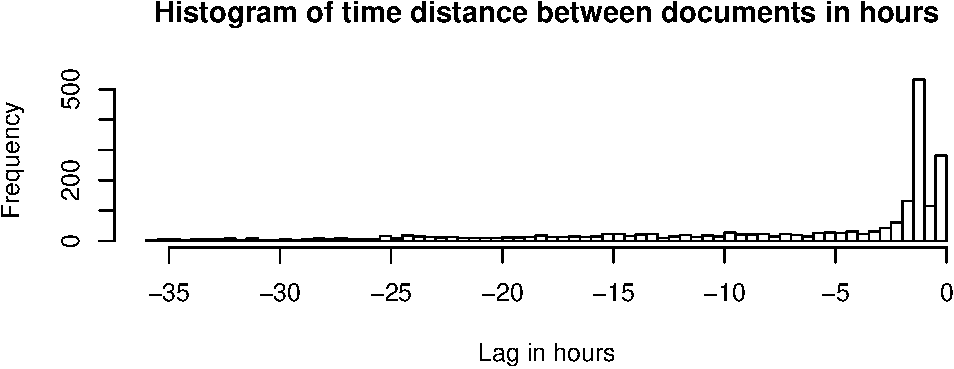
\includegraphics{newsflow_files/figure-latex/unnamed-chunk-10-1}
\textbackslash{}end\{Schunk\}

In the histogram we see that most document pairs with a similarity score
above the threshold are about an hour apart (-1 on the x-axis). This is
mainly because the online newspapers often follow the news agency within
a very short amount of time. As time distance increases, the number of
document pairs decreases, which makes sense because news gets old fast,
so news diffusion should occur within a limited time after publication.

If the goal of the document comparison is to analyze news diffusion
patterns, then there is one more thing to account for. If news diffuses
from one news outlet to another, then the time difference cannot be
zero, since the news outlet that follows needs time to edit and publish
the news. This delay period can also differ between news outlets.
Websites can adopt news within minutes, but newspapers have a long time
between pressing and publishing the newspaper, meaning that there is a
period of several hours before publication during which influence is not
possible. To make it more convenient to tailor (and store) the lag
settings for each news outlet, we made the
\texttt{source.window.settings} and \texttt{filter.lag} functions.

The \texttt{source.window.settings} function creates a data.frame that
contains for each source the minimum and maximum amount of lag.
Alternatively, if the meta information also contained another relevant
grouping attribute such as source type, this can also be used, as we'll
demonstrate.\\In the following example the minimium and maximum lag is
set to 0.1 and 36 hours, respectively. For print newspapers, the minimum
lag is then manually set to 6 hours to account for their publication
delay.\footnote{Note that the \texttt{source.window.settings} function
  also has a \texttt{direct.edit} parameter, which invokes a text editor
  to make manual adjustments.}

\begin{Schunk}
\begin{Sinput}
source.window = source.window.settings(g, max.window.left = -36, max.window.right = -0.1, 
                                       meta.attribute='sourcetype')
source.window$window.right[source.window$sourcetype == 'Print newspapers'] = -6
source.window
\end{Sinput}
\begin{Soutput}
#>          sourcetype window.left window.right
#> 1      Newsagencies         -36         -0.1
#> 2 Online newspapers         -36         -0.1
#> 3  Print newspapers         -36         -6.0
\end{Soutput}
\end{Schunk}

The advantage of this approach is that the source window data.frame can
now easily be stored for future reference. Next, \texttt{filter.lag}
uses the data.frame to filter the data in the network. Also, to display
the actual range of the window for each source, the
\texttt{show.source.window} function can be used.

\begin{Schunk}
\begin{Sinput}
g = filter.window(g, source.window)
show.window(g)
\end{Sinput}
\begin{Soutput}
#>               source window.left window.right
#> 1         Newsagency         -35        -0.15
#> 2 Newspaper 1 online         -36        -0.10
#> 3  Newspaper 1 print         -36        -7.02
#> 4 Newspaper 2 online         -36        -0.12
#> 5  Newspaper 2 print         -35        -7.35
\end{Soutput}
\end{Schunk}

Note that currently we are only comparing documents to prior documents.
This way, we focus the analysis on whether each document is potentially
influenced by certain other documents. By changing the window setting,
it is also possible to compare each document to both prior and future
documents, to focus on content homogeneity. Or to compare only to future
documents, to focus the analysis on whether each document potentially
influenced other documents.

\subsection{Aggregating and visualizing the document similarity
network}\label{aggregating-and-visualizing-the-document-similarity-network}

Before we aggregate the network, it can be informative to look at the
individual components. That is, disconnected parts of the network
consisting of one or more documents that are only similar to each other.
With the current data, these components tend to reflect documents that
address the same or related events. To inspect components, we can use
the \texttt{plot.document.network} function. This function draws a
network where nodes (i.e.~documents) are positioned based on their date
and time (x-axis) and source (y-axis). If an integer is given as an
argument for the subcomp parameter, then this specific subcomponent is
visualized and returned. Without the subcomp parameter the entire
network will be plotted, which is only useful with smaller graphs. If a
DTM is also provided, the visualization will include a word cloud with
the common words of these documents. Also, the source attribute can be
changed to other interesting meta attributes such as source type.

\begin{Schunk}
\begin{Sinput}
## Visualize and extract individual components of the network 
sg2 = plot.document.network(g, subcomp = 2, dtm=dtm)
\end{Sinput}

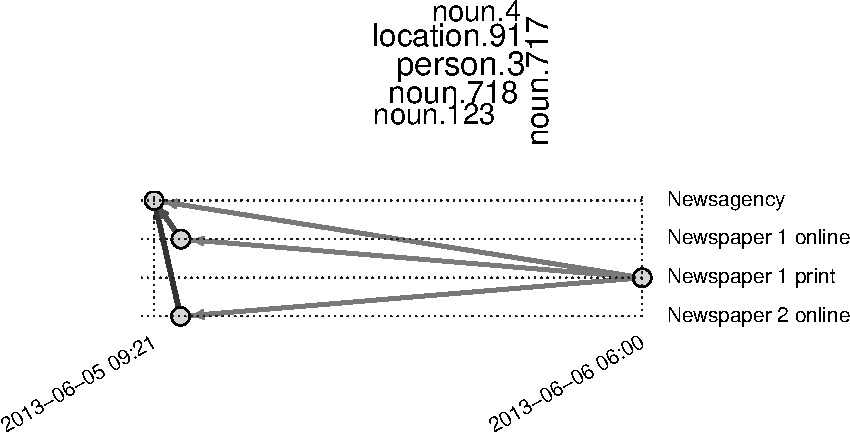
\includegraphics{newsflow_files/figure-latex/unnamed-chunk-13-1} \end{Schunk}

\begin{Schunk}
\begin{Sinput}
sg2_sourcetype = plot.document.network(g, subcomp = 2, source.attribute = 'sourcetype')
\end{Sinput}

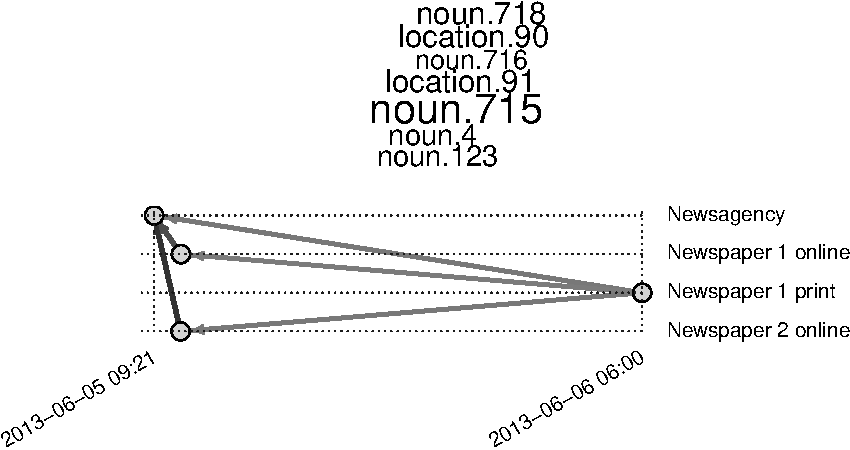
\includegraphics{newsflow_files/figure-latex/unnamed-chunk-14-1} \end{Schunk}

The first visualization (per source) shows that a news message was first
published by the news agency on June 6th, and adopted the same day by
two online newspapers, and also that one newspaper later on published an
update or follow-up item. Note that the subcomponents are also stored as
separate networks \texttt{sg1} and \texttt{sg2}, so that they can be
inspected more specifically.

These visualizations illustrate how we can analyze homogeneity and news
diffusion patterns. For each source we can count what proportion of its
publications is similar to earlier publications by specific other
sources. We can also analyze the average time between publications.

The \texttt{aggregate.network} function performs these calculations by
aggregating the edges in the network based on the vertex attributes
(i.e.~the meta information). The first argument is the \texttt{igraph}
network. The arguments for \texttt{by.from} and \texttt{by.to} are
character vectors to indicate one or more vertex attributes. This gives
flexible control over the data, for instance to analyze source to source
influence, or source to sourcetype, or to analyze per month (after
adding month as a vertex attribute). By default, the function returns
the number of edges, as well as the number of nodes that is connected
for both the \texttt{from} and \texttt{to} group. In addition, an
\texttt{edge.attribute} can be given and a function to aggregate this
attribute. For this example we use this to analyze the median of the
\texttt{hourdiff} attribute.

\begin{Schunk}
\begin{Sinput}
source_to_source = aggregate.network(g, by.from = 'source', by.to='source', 
                                     edge.attribute='hourdiff', agg.FUN=median)
s.type_to_s.type = aggregate.network(g, by.from = 'sourcetype', by.to='sourcetype', 
                                     edge.attribute='hourdiff', agg.FUN=median)

## Table printed in two parts due to width
head(s.type_to_s.type[,1:7])
\end{Sinput}
\begin{Soutput}
#>     from.sourcetype     to.sourcetype edges agg.hourdiff from.matched
#> 1      Newsagencies      Newsagencies   124         -8.1           95
#> 2 Online newspapers      Newsagencies   830         -1.3          714
#> 3  Print newspapers      Newsagencies    98        -16.1           79
#> 4      Newsagencies Online newspapers   180         -5.6          114
#> 5  Print newspapers Online newspapers   155        -15.1           86
#> 6 Online newspapers Online newspapers   379         -1.8          291
#>   from.N from.prop
#> 1    597      0.16
#> 2    879      0.81
#> 3    278      0.28
#> 4    597      0.19
#> 5    278      0.31
#> 6    879      0.33
\end{Soutput}
\begin{Sinput}
head(s.type_to_s.type[,c(1:4, 8:10)])
\end{Sinput}
\begin{Soutput}
#>     from.sourcetype     to.sourcetype edges agg.hourdiff to.matched to.N
#> 1      Newsagencies      Newsagencies   124         -8.1        112  597
#> 2 Online newspapers      Newsagencies   830         -1.3        543  597
#> 3  Print newspapers      Newsagencies    98        -16.1         89  597
#> 4      Newsagencies Online newspapers   180         -5.6        158  879
#> 5  Print newspapers Online newspapers   155        -15.1        143  879
#> 6 Online newspapers Online newspapers   379         -1.8        334  879
#>   to.prop
#> 1    0.19
#> 2    0.91
#> 3    0.15
#> 4    0.18
#> 5    0.16
#> 6    0.38
\end{Soutput}
\end{Schunk}

The default output is a data.frame where the edges of each unique
combination of the \texttt{from} and \texttt{to} groups are aggregated.
For example, we see that online newspaper documents have 830 edges to
news agency documents that were published within the previous 36 hours.
The median of the difference in hours of these documents is -1.3 (1 hour
and 18 minutes). The \texttt{from.matched} column indicates the number
of unique online newspaper documents that matched with a news agency
document\footnote{Note that the \texttt{edges} score can be higher (but
  not lower) than the \texttt{from.matched} score, since one document
  can match with multiple other documents.}. The \texttt{from.N} column
indicates the total number of online newspaper documents, and
\texttt{from.prop} is the proportion of online newspaper documents that
matched with a news agency document. Substantially, the
\texttt{from.prop} score thus indicates that 81.23\% of political news
in online newspapers is similar or identical to recent news agency news.
This indicates that online newspapers rely heavily on the news agency as
a source of political news.

The \texttt{matched}, \texttt{N} and \texttt{prop} scores are also
reported for the \texttt{to} group. This gives an interesting inversed
perspective on the relation between online newspapers and news agencies.
Based on the \texttt{to.prop} score, we see that 90.95\% of political
news published by the news agency is similar or identical to future
online newspaper news. If a news agency publishes a political news item,
it is very likely that this item will soon after be published by at
least one online newspaper. Thus note that \texttt{from.prop} and
\texttt{to.prop} are related but different scores, and can be used
complementary or to answer different research questions.

In the current aggregation we looked at all edges, but depending on the
purpose of the analysis it can be relevant to filter first. For
illustration, look again at the first visualization of the subcomponent.
Here the publications of \texttt{Newspaper 1 online} match previous
publications of both the news agency and the other online newspaper. If
we are specifically interested in who the original source of the news
is, then it makes sense to only count the edges to the news agency. This
package therefore offers the \texttt{only.first.match} function, which
will transform the network so that each document can only have 1 edge:
to the earliest dated document it matches within the specified time
window.

To demonstrate how this affects the results, we compare the previous
aggregation with an aggregation of the transformed network. For this, we
also demonstrate the \texttt{return.network} parameter of the
\texttt{aggregate.network} function, which returns the output as an
\texttt{igraph} network. For the edge weight we use the
\texttt{from.prop} score. We plot both networks, using a threshold of
0.05 for the proportion score for the sake of parsimony.

\begin{Schunk}
\begin{Sinput}
g2 = only.first.match(g)
permed.g1 = aggregate.network(g, by.from='source', by.to='source', 
                              return.network = T, network.edge.weight = 'from.prop')
permed.g2 = aggregate.network(g2, by.from='source', by.to='source', 
                              return.network = T, network.edge.weight = 'from.prop')

permed.g1 = delete.edges(permed.g1, which(E(permed.g1)$weight < 0.05))
permed.g2 = delete.edges(permed.g2, which(E(permed.g2)$weight < 0.05))

par(mfrow = c(1,2))
plot(permed.g1, layout=layout.circle, vertex.label.dist=0.6, edge.label.cex = 0.7)
plot(permed.g2, layout=layout.circle, vertex.label.dist=0.6, edge.label.cex = 0.7)
\end{Sinput}

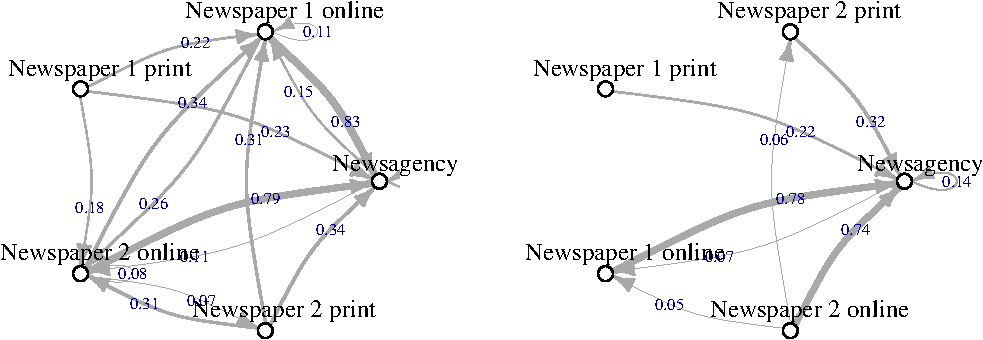
\includegraphics{newsflow_files/figure-latex/unnamed-chunk-16-1} \end{Schunk}

The first network is much more dense compared to the second. In
particular, we see stronger edges between the print and online editions
of the newspapers. In the second network almost only the ties to the
news agency remain. This implies that many of the edges between
newspapers result from cases where both newspapers adopt the same news
agency articles.

Note that the second network is not better per se. Consider, for
instance, that a blog might most of its information from an online
newspaper, in which case the news agency is often still the initial
source, but the newspaper is a crucial gatekeeper. Depending on the
purpose of the analysis, either approach can thus be more suitable.

Finally, a useful alternative way to organize the data is as a
data.frame that shows for each document whether and if so how strongly
it matches with other sources. For this we can use the
\texttt{topSimilarities} function. The output is a data.frame where the
rows represent unique documents. For each document the score for the
strongest match to each other source is given (or zero if no match is
found). In this format the data can easily be matched to data on content
characteristics of individual documents.

\begin{Schunk}
\begin{Sinput}
topsim = topSimilarities(g, break.by='sourcetype')
head(topsim,4)
\end{Sinput}
\begin{Soutput}
#>         id                date Newsagencies Online newspapers
#> 1 97359230 2013-06-01 10:52:00            0                 0
#> 2 35621313 2013-06-01 11:59:00            1                 0
#> 3 36156099 2013-06-06 04:41:00            1                 0
#> 4 97362434 2013-06-06 02:03:00            0                 0
#>   Print newspapers
#> 1                0
#> 2                0
#> 3                0
#> 4                0
\end{Soutput}
\end{Schunk}

\subsection{Conclusion and future
improvements}\label{conclusion-and-future-improvements}

We have demonstrated how the \emph{newsflow} package can be used to
perform a many-to-many comparison of documents. The primary focus and
most important feature of this package is the
\texttt{documents.window.compare} function. This function compares all
documents that occur within a given time distance, which makes it
computationally feasible for longitudinal data. Using this data, we can
analyze to what extent different sources publish the same content and
whether there are consistent patterns in who follows whom. The secondary
focus of this package is to provide functions to conduct this analysis,
and to provide a platform for scholars to share additional or
alternative approaches.

The data input required for this analysis consists solely of textual
documents and their corresponding publication date and source. If the
texts are imported as natural language, the \texttt{tm} package or
\texttt{RTextTools} package can be used to preprocess them and to create
a DTM. If the texts are imported as preprocessed tokens, the
\texttt{create.dtm} function can be used to create a DTM. Since no human
coding is required, the package enables large scale comparative and
longitudinal studies. Although the demonstration in this paper used a
moderate sized dataset, the functions can handle much larger data
\footnote{A test showed that on a laptop with 8Gb RAM and a 1.80GHz
  processor (no multi-threading used) the analysis performed well with a
  DTM containing 315.000 documents and 120.000 unique terms. This data
  covered 1 year in 14 sources, and a window of 3 days and threshold of
  0.4 was used.}.

The goal is to continue developing this package as a specialized toolkit
for analyzing the homogeneity and diffusion of news content. First of
all, additional approaches for measuring whether documents are related
will be added. Currently only a vector space model approach for
calculating document similarity is implemented\footnote{This is because
  we currently rely on matrix multiplication as a computationally
  efficient way to calculate inner-product based similarity scores, such
  as cosine similarity.}. For future versions alternative approaches
such as language modeling will also be explored. In particular, we want
to add alternative measures to express the relation of documents over
time in terms of probability and information gain. This would also allow
us to define a more formal way to determine whether or not a relation
exists, other than using a similarity threshold. Secondly, new methods
for analyzing and visualizing the network data will be explored. In
particular, methods will be implemented for analyzing patterns beyond
dyadic ties between news outlets, building on techniques from the field
of network analysis.

Ultimately, the goal is to extract communication networks from content
data for many sources over time. This package contributes to this goal
by facilitating different approaches for creating and aggregating the
document network.

\section{References}\label{references}

\bibliography{references}

\address{
Kasper Welbers\\
VU University Amsterdam\\
De Boelelaan 1081,\\ 1081 HV Amsterdam, The Netherlands\\
}
\href{mailto:k.welbers@vu.nl}{\nolinkurl{k.welbers@vu.nl}}

\address{
Wouter van Atteveldt\\
VU University Amsterdam\\
De Boelelaan 1081,\\ 1081 HV Amsterdam, The Netherlands\\
}
\href{mailto:wouter@vanatteveldt.com}{\nolinkurl{wouter@vanatteveldt.com}}

